\chapter{Optimized Heterogeneous Scheduling\\Driven by State-Transition Graphs}
\label{chap:optimizedHeterogeneousScheduling}

We are now ready to describe our optimized heterogeneous scheduler. First we provide the necessary background on state-transition graphs, which are the core of our scheduler, with Section~\ref{sec:programStg} discussing the case of a single program, Section~\ref{sec:joint_graph} describing the composition of graphs for multiple programs, and Section~\ref{sec:schedulingProcedure} summarizes the overall scheduling decisions mechanism. 


\section{Step 1: Individual program schedules}
\label{sec:programStg}

To represent all possible execution schedules for a given program we use a state-transition graph (STG). Graph states correspond to different allocation scenarios of heterogeneous hardware to program blocks. A simple graph example is provided in Fig.~\ref{fig:P2STG}, which corresponds to the $P_2$ program with execution requirements from Table~\ref{tab:demandExample}. Next we formalize the notion of such a state-transition graph.

\begin{figure*}
\center
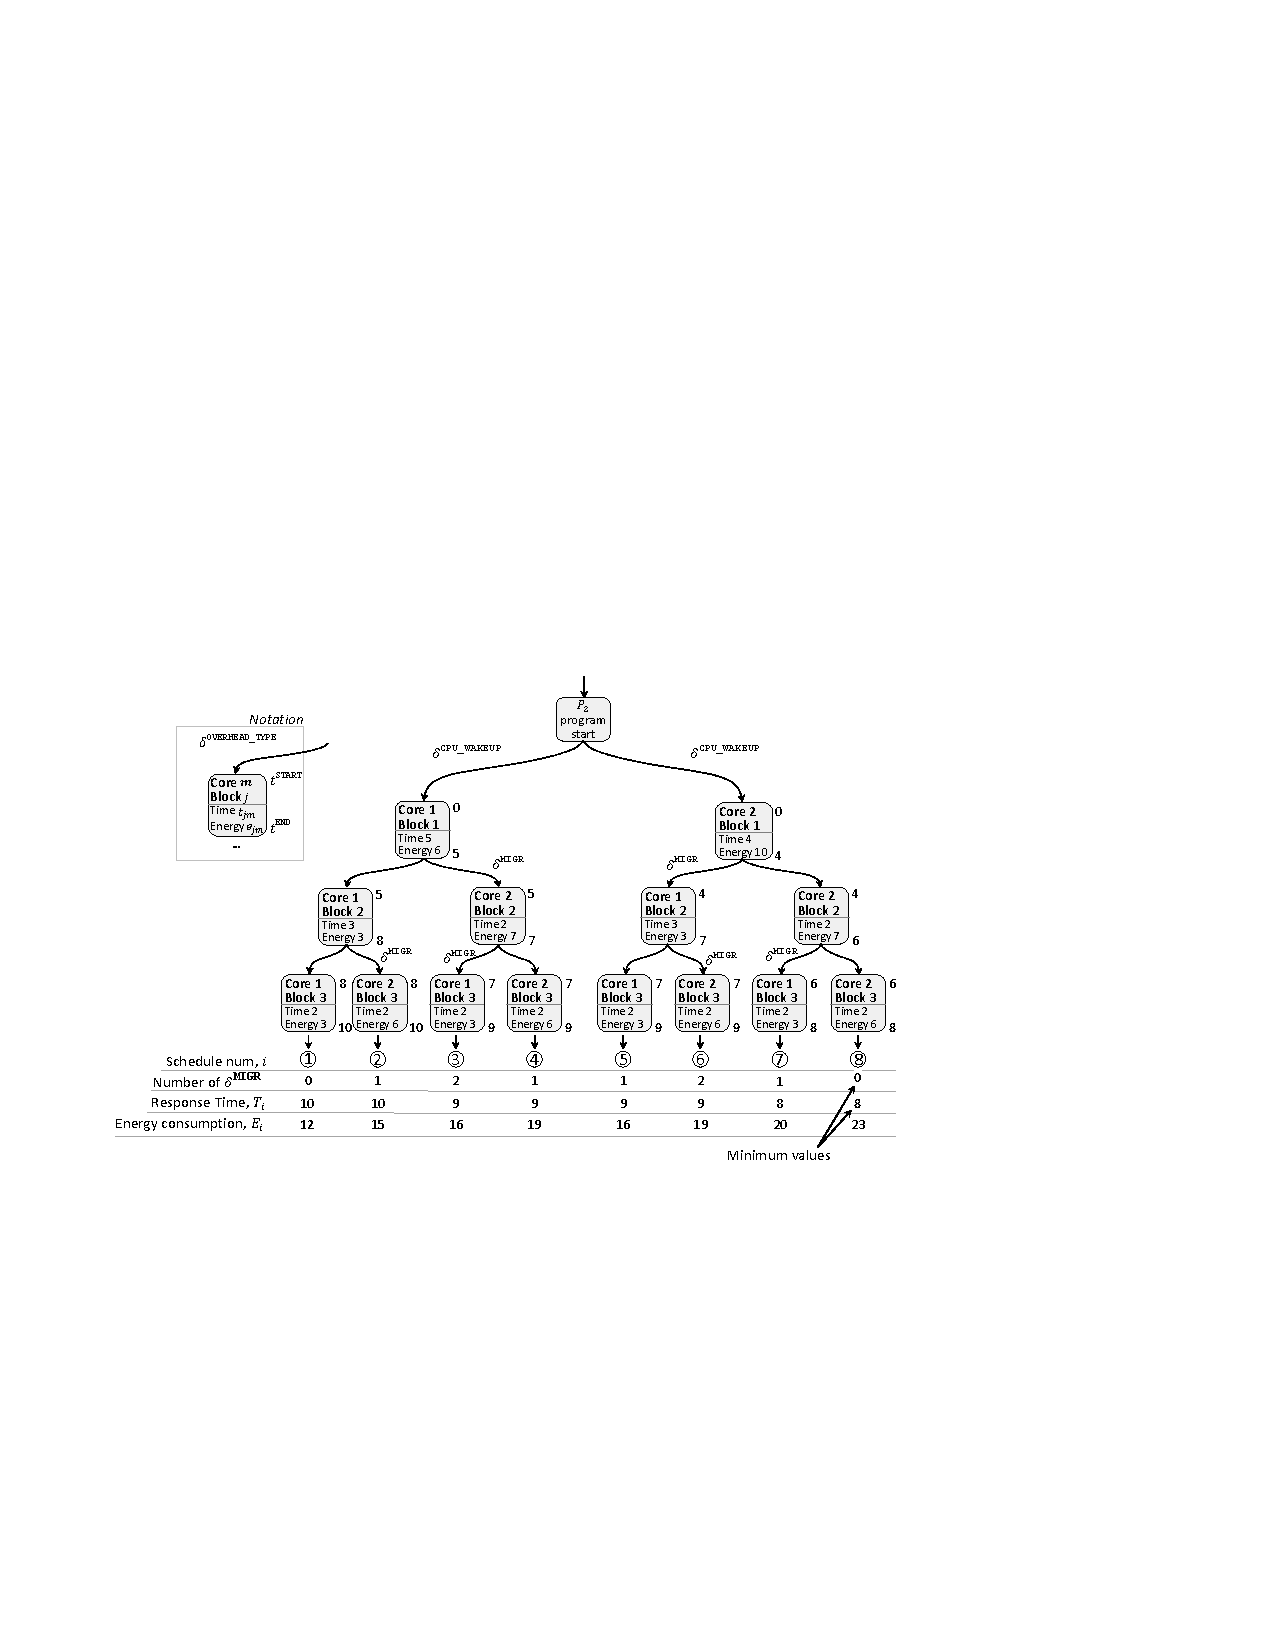
\includegraphics[width=0.95\textwidth]{figs/P2STG.pdf}
\caption{The state-transition graph of the program $P_2$ from  Table~\ref{tab:demandExample}}
\label{fig:P2STG}
\end{figure*}

Consider a program of $n$ blocks, denoted by $P = [b_1,\ldots,b_n]$.
Formally, its state-transition graph is defined according to the next principles.

\textbf{Graph state} is a tuple:
%
\begin{equation}
x = \left(m, \, j^\mathsf{block}, \, t^\mathsf{start}, \, t^\mathsf{end} \right),
\label{eq:graphState}
\end{equation}
%
where:
%
\begin{enumerate}
\item $m \in \{1,\ldots,\mathcal{M}\}$ is an allocated core type;
\item $j^\mathsf{block} \in \{1,\ldots,n\}$ is index of an executing block;
\item $t^\mathsf{start}, t^\mathsf{end}$ are start and end times of an interval allocated for block execution, counted from the initial state start.
\end{enumerate}


\textbf{Graph transition} defines, for a given state $x$, a set $\hat{X}(x)=\{\hat{x}_1, \ldots, \hat{x}_\mathcal{M}\}$ of its reachable successors\footnote{For briefness, the term ``successors" refers to ``neighbor successors"}, which is computed by:
%
\begin{equation}
\begin{aligned}
\hat{x}_m \in \hat{X}(x) \\
\forall m \in \{1,\ldots,\mathcal{M}\}
\end{aligned}
\iff
%
\begin{cases}
\hat{j}^\mathsf{block} = j^\mathsf{block} +1\\
\hat{t}^\mathsf{start} = t^\mathsf{end}\\
\hat{t}^\mathsf{end} = \hat{t}^\mathsf{start} + \left(t^\mathsf{end} - t^\mathsf{start}\right)
\end{cases}
\end{equation}
%
Set $\hat{X}$ construction is similar to \cite{Burmyakov2015}.

The execution requirements for time $t_{jm}$ and energy use $e_{jm}$ are derived from $t^\mathsf{start}$ and $t^\mathsf{end}$ as following:
%

\begin{minipage}{0.35\columnwidth}
\smallskip
\begin{equation}
t_{jm} = t^\mathsf{end} - t^\mathsf{start},
\end{equation}
\smallskip
\end{minipage}%
\begin{minipage}{.35\columnwidth}
\smallskip
\begin{equation}
e _{jm}= \frac{t^\mathsf{end} - t^\mathsf{start}}{T_{jm}}*E_{jm}
\end{equation}
\smallskip
\end{minipage}
%
Above, $T_{jm}$ and $E_{jm}$ are initial time and energy requirements of block $j^\mathsf{block}$ to be executed over an $m$-type core.  


\textbf{Graphical notation} for visualisation, also shown in Fig. \ref{fig:P2STG}, is the following:
%
\begin{itemize}
\item States are represented by rectangles with curved angles;
\item The state at the top having an incoming arrow is a program initial state, which precedes execution start;
\item Curved lines between states are transitions corresponding to some scheduling events;
\item $\delta^{\mathsf{overhead\_type}}$, which is placed near a transition arrow, denotes some performance overhead caused by this transition, e.g. due to migrations between cores.
\end{itemize}
%
For more descriptive representation, we also show $t_{jm}$ and $e_{jm}$, which are derived from math notation above.

%In turn, transitions between states represent various scheduling events, including
%%
%\begin{itemize}
%\item A core waking up or turning down;
%\item Execution start or completion of a block;
%\item Migration between processing units;
%\item Preemption by other program, in case of preemptive scheduling.
%\end{itemize}

The state-transition graph of an individual program $P$ assumes an entire hardware platform to be dedicated to the execution of exactly this program $P$ with no concurrent competitors considered. In fact, the state-transition graph is a very flexible and extensible method for modeling various scheduling problems~\cite{Burmyakov2021}.

\textbf{A program schedule} is  a graph branch from the initial state to some leaf state. In case of $k$ branches a set of schedules $\mathcal{S}$ for an $n$-block program's STG is defined as following:
%
\begin{equation}
\mathcal{S}=\{ s_1,s_2,\ldots,s_k\}
\end{equation}
%
Considering that every graph state corresponds to a certain program block execution, we say that some schedule $s_k$ is a sequence of block states:
\begin{equation}
s_k = \left[x_k(b_1),x_k(b_2),\ldots,x_k(b_n)\right]
\end{equation}
%
where each block state $x_k(b_j)$ is defined by~(\ref{eq:graphState}).

  


\section{Step 2: A merged state-transition graph}
\label{sec:joint_graph}

Typically multiple programs execute concurrently over a shared heterogeneous platform. In this case the scheduling problem is to determine an efficient allocation of heterogeneous processing units to those programs, according to chosen scheduling objectives. Moreover, it must be considered that programs arrive asynchronously and their execution over the same processing unit yields different performance gain: for example, a matrices multiplication program executes drastically faster over a GPU, while strongly sequential non-parallelisable programs typically do not benefit from GPU use in any way, despite its computational power and provided parallelism.

For our efficient scheduling we model possible concurrent executions of given programs. For such modeling we merge STGs of individual programs into a so-called joint state-transition graph (jSTG). An example of a simple jSTG is depicted in Fig.~\ref{fig:jSTGExample}, and its formal description is given below.

\textbf{Graphs state} of a jSTG, called a system state, is a set of program states $\mathcal{P} = \{y_1,\ldots,y_N\}$. Each program state $y_k$ is a tuple similar to a state $x$ of an individual program's STG described above, i.e. describes an execution of a program block $x.j^{block}$. The state represents an entire or partial block $y_k.j^{block}$ execution. In case of the entire execution, a program state is the same as a state in its STG.  In case of partial execution, a program state spreads across $l$ consequent system states $Y$ such that the core type $y.m$ is the same $\forall y \in Y$ and $\sum_{k=1}^l{y_k.t^{end}-y_k.t^{start}}=T_{y_k.j^{block},m}$, i.e. the overall time allocated to block $j$ execution equals to required time for an $m$ type core.

Overall, the jSTG state $y_k(\mathcal{P})$ of a programs state set $\mathcal{P}=\{x_1,\ldots,x_N\}$ is defined as following:
%
\begin{equation}
\begin{aligned}
y_k(\mathcal{P}) = \{x_1,\ldots,x_N\} \iff x_a.m_{l1} \neq x_b.m_{l2} \\
\forall l1,l2 \in \{1,\ldots,\mathcal{M}\}\ |\ l1 \neq l2
\end{aligned}
\label{eq:jGraphState}
\end{equation}
%

%\textbf{Graph transition} defines, for a given state $\mathcal{p}$ of $N$ programs, a set $\hat{P}(p)$

\textbf{Graphical notation} of jSTG depicted in Fig.~\ref{fig:jSTGExample} provides:
\begin{enumerate}
\item Top black circle \-- the initial state;
\item Dashed rectangles \-- combined program states\footnote{The programs set excludes programs without an allocated core};
\item Horizontal dashed lines \-- programs arrivals;
\item ``Idle" keywords \-- no-program state;
\item Paths from initial state to graph leafs \-- schedules..
\end{enumerate}
The color of program states distinguishes programs, which corresponds to programs colors in Fig.~\ref{fig:twoSchedulesExample}.  The example illustrates schedules S1 and S2 from Fig.~\ref{fig:twoSchedulesExample}.

\begin{figure*}
\center
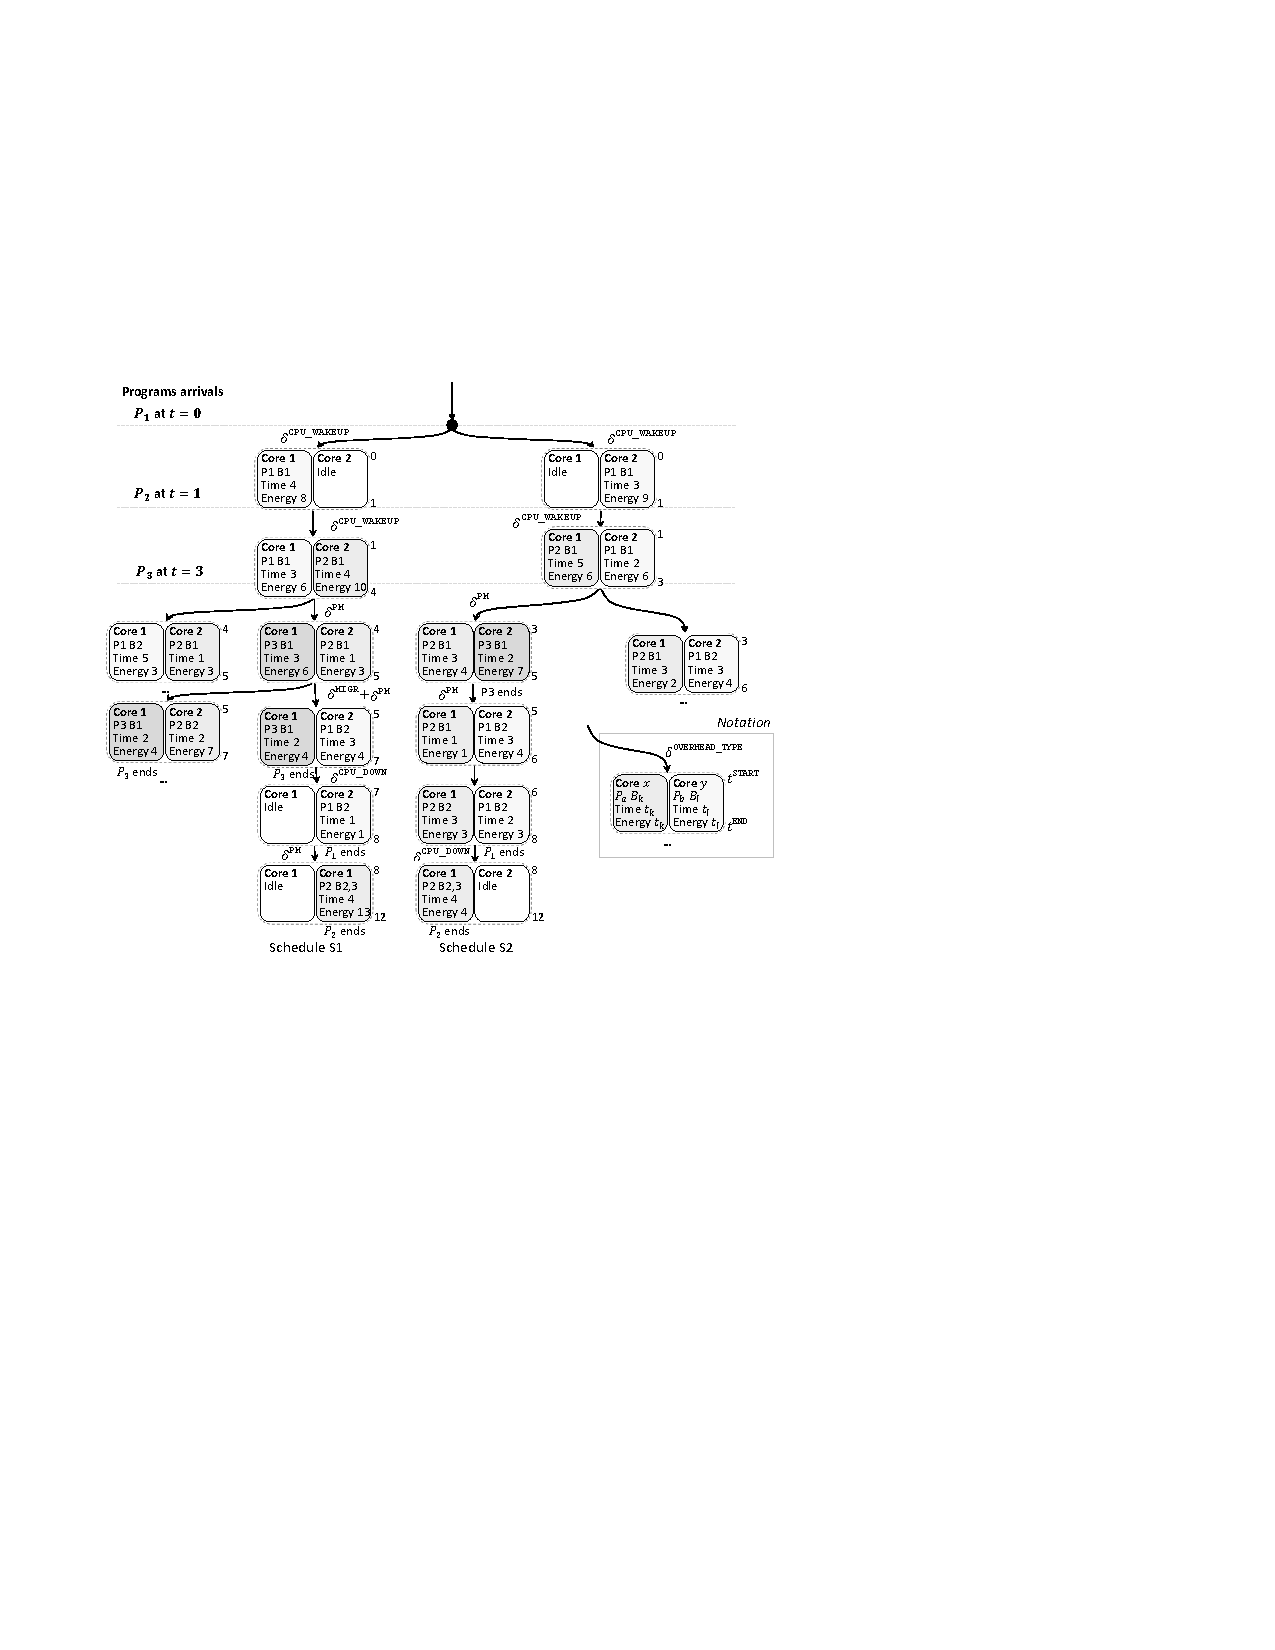
\includegraphics[width=.9\textwidth]{figs/jSTG.pdf}
\caption{A joint state-transition graph with schedules from Fig.~\ref{fig:twoSchedulesExample}. The case of non-preemptive scheduling.}
\label{fig:jSTGExample}
\end{figure*}

The joint state-transition graph of concurrent programs assumes:
%
\begin{itemize}
\item An entire heterogeneous platform is available;
\item A single core executes at most one program at a time;
\item Performance overheads are insignificant.
\end{itemize}
%
The example with three programs is directly extendable to multiple concurrent programs by analogy.

The graph in Fig.~\ref{fig:jSTGExample} models the execution of three programs $P_1$, $P_2$, $P_3$, with their parameters listed in Table~\ref{tab:demandExample} over $m=2$ core types. Observe that programs arrive asynchronously at time instants $t=0,\,1,$ and $3$.

\textbf{A schedule} for a joint-STG represents a sequence of graph system states. Where a system state is a set of program states defined above. A set of such schedules $\mathcal{S}^\mathsf{joint}$ is defined by:
%
\begin{equation}
\mathcal{S}^\mathsf{joint}=\{ s_1^\mathsf{joint}\ldots,s_k^\mathsf{joint}\}
\end{equation}
%
Considering a single schedule $s^\mathsf{joint}_k$ to be a sequence of $l$ system states for a set of programs $\mathcal{P}=\{p_1,\ldots, p_N\}$. Such a sequence is defined as follows:
%
\begin{equation}
s^\mathsf{joint}_k = \left[y_{1,k}(\mathcal{P}),\ldots,y_{l,k}(\mathcal{P})\right]
\end{equation}
%
where $y_l,k(\mathcal{P})$ is a graph system state defined in~(\ref{eq:jGraphState}).




%\section{Step 3: Allocation of processing units}
%\label{sec:optimized_scheduling_decisions}


\section{Scheduling procedure: Putting the pieces together}
\label{sec:schedulingProcedure}

\begin{figure}
\center
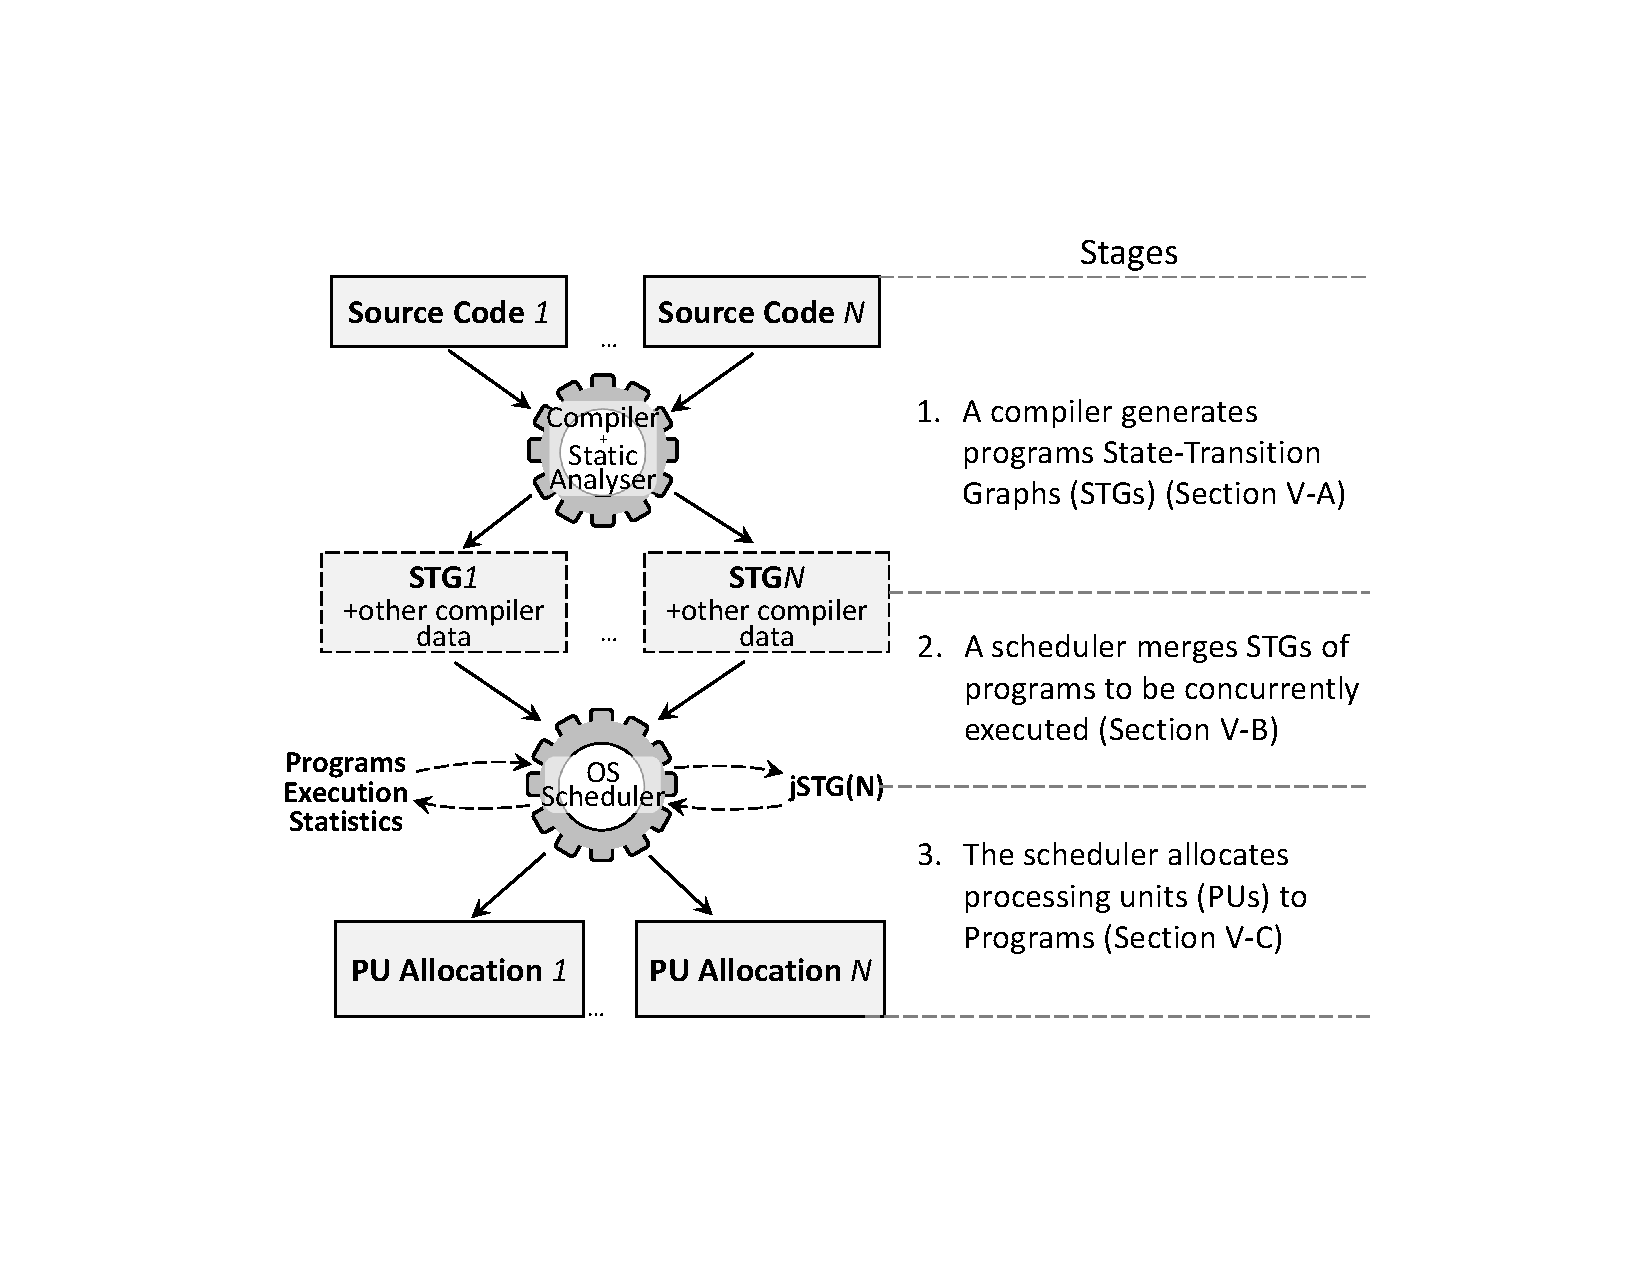
\includegraphics[width=.8\columnwidth]{figs/compilerAssistedSchedulingConcept.pdf}
\caption{Proposed extension to heterogeneous scheduling}
\label{fig:compilerAssistedSchedulingConcept}
\end{figure}

We are finally ready to formalize the procedure of our optimized heterogeneous scheduling. Its key steps are outlined in Fig.\ref{fig:compilerAssistedSchedulingConcept} and are the following:

\begin{itemize}
\itemindent=26pt
\item[\emph{Step 1:}] A compiler generates STGs from programs source code (Section~\ref{sec:programStg});
\item[\emph{Step 2:}] A scheduler merges STGs of programs to be concurrently executed (Section~\ref{sec:joint_graph});
\item[\emph{Step 3:}] The scheduler allocates processing units to programs based on the constructed joint-STG as discussed below);
\end{itemize}
%
To make efficient heterogeneous sheduling decisions, a scheduler analyzes total response times and energy consumptions of different execution schedules\footnote{The schedules examination procedure can be optimized with state-space pruning techniques \cite{Burmyakov2022}, which avoids non-optimal transitions in a state-transition graph},
%
which are illustrated below in Fig.~\ref{fig:P2STG}. An operating system scheduler then examines summaries of these schedules aiming at an optimal trade-off between schedule response time and energy consumption, which is discussed in Section~\ref{sec:energyDelayProduct}. 
